\documentclass[letterpaper,twocolumn,10pt]{article}
\usepackage{usenix2019_v3}

\usepackage{tikz}
\usepackage{amsmath}
\usepackage{graphicx}
\usepackage{comment}
\usepackage{xcolor}
\usepackage{amsfonts}
\newcommand\todo[1]{\textcolor{red}{#1}}

\graphicspath{ {./images/} }

\begin{document}
\title{\Large \bf Clustering Research for Hierarchical and Autonomous Fog Architecture}

\author{
{\rm Robin C.\ Ward}\\
PhD Student\\
Auburn University\\
Auburn, Alabama 36849\\
Email: rcw0024@auburn.edu\\
Last Edit: \today
}

\maketitle

\begin{abstract}
Our population is increasing rapidly(there is approximately a net gain of one new person on the planet Earth every 31 seconds\footnote{\url{https://www.census.gov/popclock}}), and the need to manage all of those new devices coming online will grow with it. Thankfully, HAFA~\cite{10.1145/3229710.3229740} was designed to handle such situations. However, when given a finite resource such as the space on planet Earth, and combine that with a growing population, clustering based on density will be very important. This paper will cover the implementation of other clustering algorithms, such as the DBSCAN~\cite{10.5555/3001460.3001507} method, into the HAFA architecture.\todo{State reasons why DBScan is particularly suitable for this architecture instead of other possible methods (list a few) of pre-clustering.}
\end{abstract}

\section{Introduction}
\todo{PUT EXPLANATION OF DBSCAN PSEUDO CODE HERE}~\ref{fig:pseudocode}
DBSCAN will accept two parameters: Eps and MinPts.

\section{Current Research}
\subsection{Use DBSCAN on first pass.}
Use DBSCAN to cluster highly dense areas within each layer. This will enable DBSCAN to cluster nodes in highly dense areas very fast, then cluster the outliers based on the Agglomerative Complete Linkage Hierarchical Clustering method. The use of DBSCAN could be based on several factors, including but not limited to: distance, MIPS, power. For example, the radius of the circle for the Core Point qualification could increase for a specific node if they are lacking certain resources and require more for specific load balancing activities. There is also the issue of finding a value for $\epsilon$. Because $\epsilon$ will denote the radius of the neighborhood, the value could therefore increase in an effort to have larger clusters if more resources are needed. One known method for finding a suitable value for Eps is mentioned in the DMDBSCAN~\cite{dmdbscan} paper. The algorithm~\ref{fig:dmdbscan} for DMDBSCAN will begin by calculating the distance to the nearest $\mathbb{N}$ point for each point in the data set. The results will then be sorted and plotted. The optimal value for Eps will be where the curve is most pronounced. In order to use link latency in this equation, one idea is to use the Propagation Time \todo{insert ref} instead of the distance in the DMDBSCAN formula. The propagation delay formula:
\begin{verbatim}
Propagation time = Distance / propagation speed 
\end{verbatim}
If Propagation Time will not work in DMDBSCAN, perhaps the Distance could be extracted and used?
 
\subsection{Using Great-circle distance vs. Euclidean.}Because earth is mostly spherical, if using a distance metric for geographic data, would it would make more sense to use Great-circle distance? \todo{need to check if this has been implemented in pFogSim or published already.}

\todo{come up with novel algorithm that combines the below ideas. i.e. combines MIPS with propagation time}

\subsection{Idea 1.} One potential idea for clustering based on MIPS would be to have a threshold of total MIPS for each cluster, which would prevent the total cluster MIPS from going over. This would enable a check to see the approximate amount of needed clusters that would be needed to meet the threshold standards set by the domain expert; then k-means clustering could be used, which is faster than DBSCAN. \todo{put pseudocode from my python tool}

\subsection{Idea 2.} \todo{Research node navigation i.e. circumvent buildings or down nodes. Look at Zoom drawing for ideas.}

\section{Potential Problems and Solutions}
This section covers possible issues that will arise during testing, as well as possible solutions.
\begin{description}
\item[DBSCAN Qualifications.] The use of DBSCAN as a first pass should only be used if it will increase the run time. Therefore, a potential check could be implemented to ensure that running DBSCAN will in fact help with the run time. For example, a city block that only has 10 devices which are spread out could have a longer run time if using the aforementioned method. However, if that same city block had 1000 devices that were tightly packed, the run time would be greatly reduced by using DBSCAN first. Because of this, a qualification algorithm could be implemented to check if DBSCAN would be beneficial or not. Obviously the run time of this check would also have to be low enough to make it worth it. Otherwise, we would just blindly run the DBSCAN every time, which could still be the better option. An example qualification algorithm could be:
\begin{verbatim}
if point_density > threshold:
 return DBSCAN + Agglomerative
else:
 return Agglomerative
\end{verbatim}
An important item to note here is there is an existing algorithm within the DBSCAN paper that covers getting $\epsilon$. This could potentially be used for finding the point density for the "precheck".
\end{description}

\section{Computational Complexity of using DBSCAN within HAFA}

\begin{description}
\item[Best-case] Best case complexity will be $O (n log n)$ vs. $O(n^3)$ of HAFA.
\item[Average-case] Average case complexity will be better.
\item[Worst-case] Worst-case complexity will remain the same as HAFA, $O(n^3)$.
\end{description}

\section{Idea Scratchpad}
On finding the value for $\epsilon$:
Perhaps for the specific fog layer or data set that is being used, some kind of check could be performed to see if the average MIPS of the nodes are at a threshold. For example, if the average MIPS are not meeting the threshold, the $\epsilon$ for DBSCAN could increase in an effort to make larger clusters. These larger clusters would allow for better load balancing due to the increased amount of hardware. Some quick pseudo-code could be:
\begin{verbatim}
# Finding a value for DBSCAN(Eps)
if AverageMIPS < threshold:
 return .3
else:
 return .2
\end{verbatim}
 The return values need work...perhaps a loop to keep increasing until the average MIPS is no longer below the threshold. This would require a different idea. This would involve a loop that checks the current MIPS within the cluster as DBSCAN runs, then if they do not meet the threshold, the Eps could increase in size to acquire more nodes. Another idea: have the MIPS per cluster be a new variable within HAFA. Then, as DBSCAN runs, it will check if it has hit that threshold, if yes, then the MinPts and Eps could drastically change so that the current clustering process ends, thus forming a new cluster.
 
 ****Will need to alter the DBSCAN algo...I think the best solution would be to begin the clustering, if cluster is complete AND the threshold is not met, then the Eps could increase to find more resources...

\begin{figure}[h]
\centering
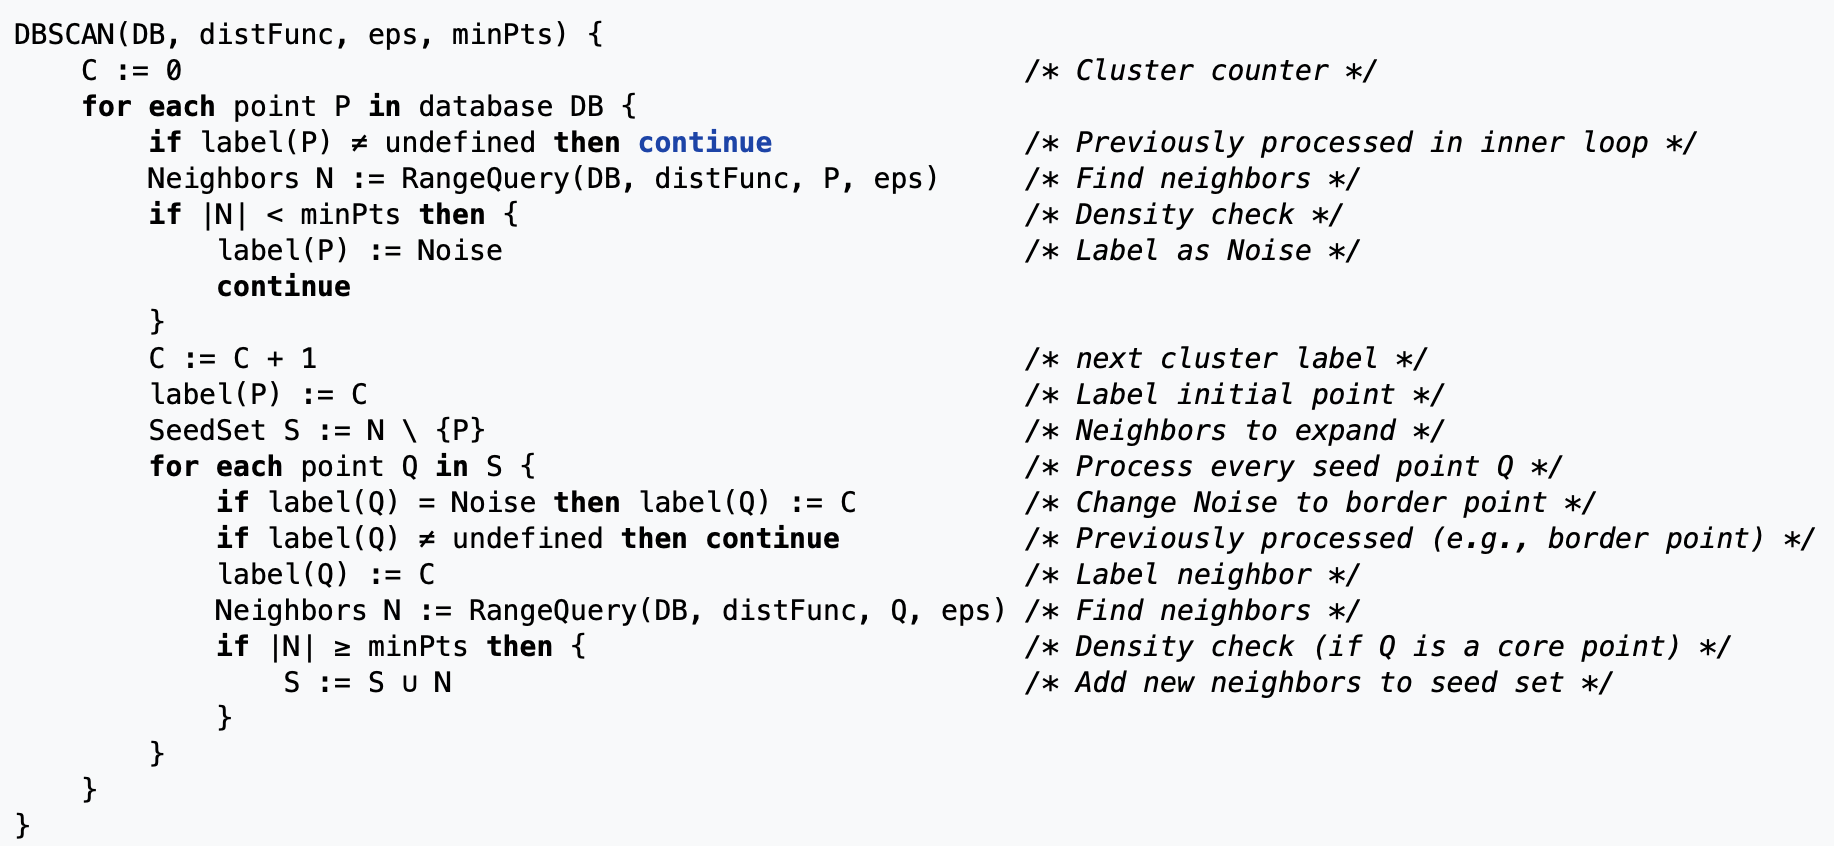
\includegraphics[width=0.45\textwidth]{pseudocode}
\caption{\label{fig:pseudocode}DBSCAN Pseudocode.}
\end{figure}

\begin{figure}[h]
\centering
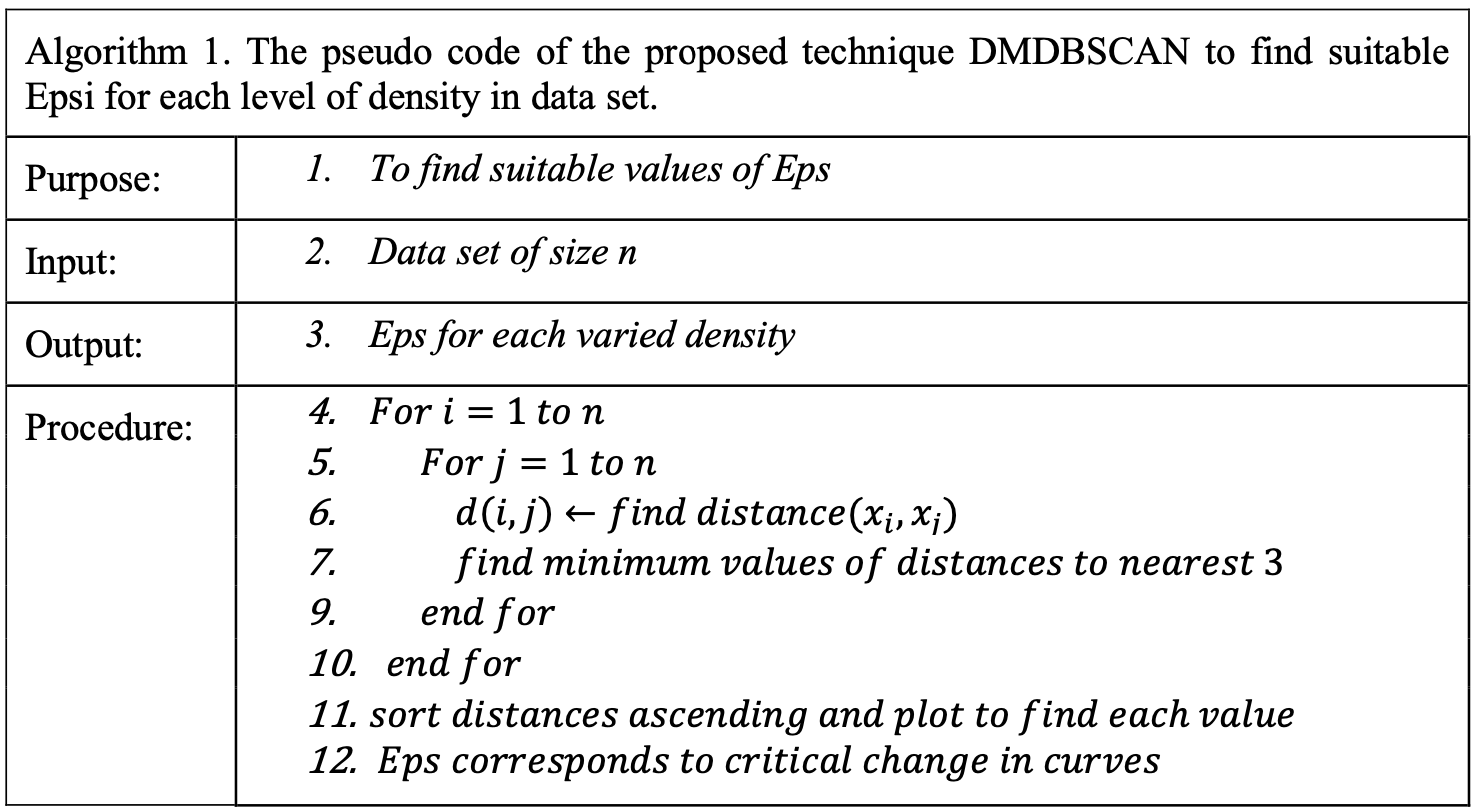
\includegraphics[width=0.45\textwidth]{dmdbscan}
\caption{\label{fig:dmdbscan}DMDBSCAN Pseudocode.}
\end{figure}

\bibliographystyle{plain}
\bibliography{bibliography.bib}
\end{document}